%%% %%%%%%%%%%%%%%%%%%%%%%%%%%%%%%%%%%%%%%%%%%%%%%%%%%%%%%%%%%%%%%%%%%%%%%%%%%
\documentclass{beamer}


% %%%%%%%%%%%%%%%%%%%%%%%%%%%%%%%%%%%%%%%%
%  Mode
% %%%%%%%%%%%%%%%%%%%%%%%%%%%%%%%%%%%%%%%%
\mode<presentation>
{
  %\usetheme[hideallsubsections]{Aachen}
  %\usetheme{Luebeck}
  \usetheme{Malmoe}
  \usefonttheme{professionalfonts}
  \useoutertheme[subsection=false, footline=authorinstitutetitle]{smoothbars}
  \usecolortheme{orchid}
  % oder ...

  \setbeamercovered{transparent}
  % oder auch nicht
}

% %%%%%%%%%%%%%%%%%%%%%%%%%%%%%%%%%%%%%%%%
%  Packages
% %%%%%%%%%%%%%%%%%%%%%%%%%%%%%%%%%%%%%%%%

\usepackage[latin1]{inputenc}
\usepackage{graphics}
\usepackage{graphicx}
\usepackage{xcolor}
%\usefonttheme[onlymath]{serif}
\usepackage{amsmath}
\usepackage{amssymb}
\usepackage{amsfonts}
%\usepackage{times}
%\usepackage[T1]{fontenc}
\usepackage{listings}
%\usepackage{psfrag}
%\usepackage{rotating}
%\usepackage{xmpmulti}
%\usepackage{pgfarrows}
%\usepackage{tabularx}
\usepackage{hyperref}
\usepackage{algorithmic}
\usepackage{float}
\usepackage{tikz}
%\usepackage{program}
%\usepackage[pst-all]{graphicx}

\tikzstyle{normalnode}=[draw,%
                          rectangle,%
                          shade,%
                          minimum size  = 1.0cm,%
                          node distance = 1.3cm]
 \tikzstyle{normalnode2}=[draw,%
                          rectangle,%
                          shade,%
                          minimum size  = 1.0cm,%
                          node distance = 1.0cm]
  \tikzstyle{normalnode3}=[draw,%
                          rectangle,%
                          shade,%
                          minimum size  = 1.0cm,%
                          node distance = 5.0cm]
  \tikzstyle{start}=[draw,fill=green!70,rectangle, minimum size=1.0cm,node distance=1.3cm]                        
  \tikzstyle{goal}=[draw,fill=red!70,rectangle, minimum size=1.0cm,node distance=1.3cm]
  \tikzstyle{goal2}=[draw,fill=red!70,rectangle, minimum size=1.0cm,node distance=1.0cm]
  \tikzstyle{agent}=[draw,fill=blue!70,circle,minimum size=0.6cm]
  \tikzstyle{dummy}=[circle]



%%%%%%%%%%%%%
\newcommand{\topalign}[1]{%
  \begin{columns}%
    \begin{column}[T]{0pt}%
      \vspace*{\textheight}%
    \end{column}%
    \begin{column}[T]{\textwidth}%
      #1%
    \end{column}%
  \end{columns}%
}


% %%%%%%%%%%%%%%%%%%%%%%%%%%%%%%%%%%%%%%%%
%  Macros/Defs
% %%%%%%%%%%%%%%%%%%%%%%%%%%%%%%%%%%%%%%%%

\colorlet{lightblue}{blue!50!white}

\def\blue#1{\color{blue}#1\color{black}}
\def\lightblue#1{\color{lightblue}#1\color{black}}
%\def\lightblue#1{\color{blue}\begin{colormixin}{10!white}#1\end{colormixin}\color{black}}
\def\red#1{\color{red}#1\color{black}}

% %%%%%%%%%%%%%%%%%%%%%%%%%%%%%%%%%%%%%%%%
%  Title Information
% %%%%%%%%%%%%%%%%%%%%%%%%%%%%%%%%%%%%%%%%
\title[Multi-Agent Reinforcement Learning]{Multi-Agent Reinforcement Learning}

\author[C.Kalla]{Christian Kalla}
\institute[RWTH Aachen University]
{ Knowledge-Based Systems Group\\
  RWTH Aachen University
}

\date[8.6.2009] % (optional, sollte der abgek�rzte Konferenzname sein)
{8.6.2009/Seminar- Foundations of AI}

\subject{Subject}

\pgfdeclareimage[height=0.5cm]{university-logo}{pics/logo_blau_rechts}
\logo{\pgfuseimage{university-logo}}


%\AtBeginSection[]
%{
 % \begin{frame}<beamer>
 %   \frametitle{Outline}
 %   \tableofcontents[currentsection,currentsubsection]
 % \end{frame}
%}

% make the title area


%% %%%%%%%%%%%%%%%%%%%%%%%%%%%%%%%%%%%%%%%%%%%%%%%%%%%%%%
%%  Begin Document
%% %%%%%%%%%%%%%%%%%%%%%%%%%%%%%%%%%%%%%%%%%%%%%%%%%%%%%%
\begin{document}


% %%%%%%%%%%%%%%%%%%%%%%%%%%%%%%%%%%%%%%%%
\begin{frame}
  \titlepage
\end{frame}
\begin{frame}
\frametitle{Overview}
\tableofcontents[pausesections]
\end{frame}

\section{Introduction}

% %%%%%%%%%%%%%%%%%%%%%%%%%%%%%%%%%%%%%%%%
\begin{frame}
  \frametitle{The Idea of Reinforcement Learning}
  \begin{itemize}
  \item learning by interacting with the environment
  \item taking actions and receiving rewards
  \item trying to maximize long-term reward
  \item mathematical description: \textcolor{red}{Markov Decision Process}
  \end{itemize}
\end{frame}
\begin{frame}
\frametitle{The Idea of Reinforcement Learning}
\begin{tikzpicture}[overlay]
\node[normalnode3] (agent) at (3,0) {Agent};
\node[normalnode3] [right of=agent] (environment) {Environment};
\path<2-3>[->] (agent.south) edge[very thick,bend right] node[below]{action} (environment.south);
\path<3-3>[->] (environment.north) edge[very thick,bend right,red] node[above]{reward, new state} (agent.north);
%\edge[pre,bend,right] (environment)
\end{tikzpicture}
\end{frame}
\begin{frame}
\frametitle{Reinforcement Learning - Some Real World Analogies}
\begin{itemize}
\item Learning to drive (without a driving instructor)
\pause
\item Infants learning to walk
\pause
\item Playing a game of chess
\pause
\item Preparing the breakfast
\pause
\item a mobile cleaning robot deciding to collect more trash or to find the way back to the recharging station
\end{itemize}
\end{frame}
\begin{frame}
\frametitle{Comparison to other Machine Learning Approaches}
\begin{itemize}
\item \textbf{Supervised Learning}
\pause
\begin{itemize}
\item given correct input-output pairs
\item correct classification of data given $\rightarrow$ \textcolor{red}{"teacher"}
\item example: digit recognition
\end{itemize}
\pause
\item \textbf{Unsupervised Learning}
\begin{itemize}
\item just "raw data" without labeling given
\item no "teacher"
\item example: clustering methods (k-means,...)
\end{itemize}
\pause
\item \textbf{Reinforcement Learning}
\begin{itemize}
\item learning by interacting with the environment
\item "natural" approach (related to human learning)
\item feedback from environment in terms of rewards
\item goal: maximize long-term reward
\end{itemize}
\end{itemize}
\end{frame}         

\section{Foundations of Reinforcement Learning}
\subsection{Markov Decision processes}
\begin{frame}
\frametitle{The Markov Property}
\begin{block}{Markov Property}
\begin{equation*}
\begin{align}
&Pr\left\{s_{t+1}=s',r_{t+1}=r| s_{t},a_{t},r_{t},s_{t-1},a_{t-1},...,r_{1},s_{0},a_{0} \right\}\\
=&Pr\left\{s_{t+1}=s',r_{t+1}=r| s_{t},a_{t} \right\}   
\end{align}
\end{equation}
\end{block}
The probability distribution of the next state only depends on the previous state and not on all the states visited before
\end{frame}
\begin{frame}
\frametitle{Markov Decision Process(MDP)}
\begin{block}{Components of an MDP}
\begin{itemize}
\item a set of states $\mathcal{S}$
\item a set of actions $\mathcal{A}$
\item a set of rewards $\mathfrak{R}$
\item a transition function $T:\mathcal{S}\times \mathcal{A}\rightarrow PD(\mathcal{S})$ where $PD(\mathcal{S})$ denotes the set of probability distribution over $\mathcal{S}$
\item a reward function $R:\mathcal{S} \times \mathcal{A} \rightarrow \mathfrak{R}$
\end{itemize}
\end{block}
\begin{alertblock}{Goal:Maximize expected sum of discounted future rewards:}
\begin{equation*}
E \left\{\sum_{j=0}^{\infty}{\gamma^{j}r_{t+j}} \right\}
\end{equation}
\end{alertblock}
\end{frame}
\begin{frame}
\frametitle{Finding a Way to the Goal}
In order to find an optimal way from the state to the goal we have to do the following:
\begin{block}{What needs to be done?}
\begin{itemize}
\pause
\item Compute/Estimate how good a state is
\begin{itemize}
\item quality of states $\rightarrow$ \textcolor{red}{value function $V(s)$}
\item quality of actions $\rightarrow$ \textcolor{red}{Q-Function $Q(s,a)$}
\end{itemize}
\pause
\item Find a method that chooses the \textcolor{red}{best action} in \textcolor{red}{every situation} $\rightarrow$ \textcolor{red}{Optimal Policy}
\end{itemize}
\end{block}
\end{frame}
\subsection{Policies}
\begin{frame}
\frametitle{Properties of Policies}
\begin{itemize}
\item Tell the agent which action to choose in each possible situation
\item may be deterministic or stochastic
\begin{itemize}
\item deterministic policies: action is clearly specified
\item actions are taken with a defined probability (necessary in many games)
\end{itemize}
\item should lead the agent to a goal state as fast as possible
\end{itemize}
\end{frame}
\begin{frame}
\frametitle{Policy- A Formal Definition}
\begin{definition}[Policy]
Let $S$ be a set of states and $A$ be a set of actions an agent can choose in its environment.\\
A mapping $\pi:S \rightarrow A \ \forall s \in S$ is called a policy .
\end{definition}
\end{frame}
\begin{frame}
\frametitle{Optimal Policy: A Formal Definition}
\begin{definition}[Optimal Policy]
A policy $\pi^{*} \in \Pi$ that maximizes the quantity
\begin{equation*}
R=r_{0}+r_{1}+...+r_{n}
\end{equation}
for Markov decesion processes with a terminal state or the quantity
\begin{equation*}
R=\sum_{t}{\gamma^{t}r_{t}}
\end{equation}
for MDPs without a terminal state ($0 \leq \gamma \leq 1$ denotes the discounting factor) is called optimal policy.
\end{definition}
\end{frame}
\begin{frame}
\frametitle{Examples for Policies}
\begin{itemize}
\item A bad deterministic policy for a grid world
\begin{center}
  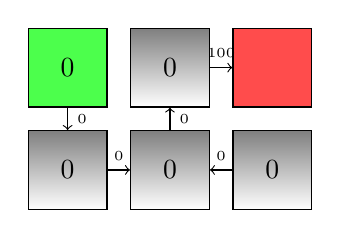
\begin{tikzpicture}
            \node[start] (a)  {0};
            \node[normalnode][right of=a]  (b) {0};
            \node[goal][right of=b]  (c) {};
            \node[normalnode][below of=a]  (d) {0};
            \node[normalnode][right of=d]  (e) {0};
            \node[normalnode][right of=e] (f) {0};
            \draw [->] (a.south) to  node[right] {\tiny 0}  (d.north);
            \draw [->] (d.east) to node[above] {\tiny 0} (e.west);
            \draw [->] (e.north) to node[right] {\tiny 0} (b.south);
            \draw [->] (b.east) to node[above] {\tiny 100} (c.west);
            \draw [->] (f.west) to node[above] {\tiny 0} (e.east);	
  \end{tikzpicture}
\end{center}
\item Optimal stochastic policy for the game Rock-Paper-Scissors: $\pi(rock)=\pi(paper)=\pi(scissors)=\frac{1}{3}$
\end{itemize}
\end{frame}
\begin{frame}
\frametitle{Policies addressing the Exploration vs. Exploitation Problem}
\begin{block}{$\epsilon$ greedy policy}
\begin{itemize}
\item choose the state-action pair with the highest value (or the action leading to the state with the highest value)
\item choose a random action with the probability $\epsilon$
\end{itemize}
\end{block}
\begin{block}{Softmax}
Select action $a$ in state $s$ with probability
\begin{equation*}
p(s,a)=\frac{e^{\frac{Q(s,a)}{\tau}}}{\sum_{a'}{e^{\frac{Q(s,a')}{\tau}}}}
\end{equation}
\end{block}
\end{frame}
\subsection{State-Value and Action-Value-Function}
\begin{frame}
\frametitle{State-Value Function}
\begin{definition}[State-value function]
The function
\begin{equation*}
V^{\pi}(s)=E_{\pi}\left\{R_{t}|s_{t}=s \right\}=E_{\pi}\left\{ \left. \sum_{k=0}^{\infty}{\gamma^{k}r_{t+k+1}}\right|s_{t}=s  \right\}
\end{equation}
is called the state-value function for policy $\pi$. $E_{\pi}{}$ =expected value assuming the agent follows the policy $\pi$ with an arbitrary time step $t$.
\end{definition}
\begin{definition}[Optimal state-value function]
The function
\begin{equation*}
V^{*}(s)=\max_{\pi}{V^{\pi}(s)} \forall s \in \mathcal{S}
\end{equation}
is called optimal state-value function.
\end{definition}
\end{frame}
\begin{frame}
\frametitle{Action-Value Function}
\begin{definition}[Action-value function]
The function
\begin{equation*}
Q^{\pi}(s,a)=E_{\pi}\left\{R_{t}|s_{t}=s, a_{t}=a \right\}=E_{\pi}\left\{ \left. \sum_{k=0}^{\infty}{\gamma^{k}r_{t+k+1}}\right|s_{t}=s, a_{t}=a  \right\}
\end{equation}
is called the action-value function for policy $\pi$. 
\end{definition}
\begin{definition}[Optimal action-value function]
The function
\begin{equation*}
Q^{*}(s,a)=\max_{\pi}{Q^{\pi}(s,a)} \forall s \in \mathcal{S}\ and \ a \in \mathcal{A}(s)
\end{equation}
is called optimal action-value funciton.
\end{definition}
\end{frame}
\subsection{Basic algorithms}
\begin{frame}
\frametitle{Categorization of RL- Algorithms}
\begin{block}{Dynamic Programming Methods}
\begin{itemize}
\item require full world knowledge (so not applicable in many cases)
\item use Bellman equation to find an optimal policy
\item have to consider a large state and action set
\end{itemize}
\end{block}
\begin{block}{Monte Carlo Methods}
\begin{itemize}
\item do not require full world knowledge
\item perform an episode and update state values and policy \textcolor{red}{afterwards}
\end{itemize}
\end{block}
\end{frame}
\begin{frame}
\frametitle{Categorization of RL- Algorithms}
\begin{block}{Temporal Difference Learning}
\begin{itemize}
\item do not require full world knowledge
\item update values of states based on values of successor states
\item distinction between \textcolor{red}{On}- and \textcolor{red}{Off}- Policy algorithms
\begin{itemize}
\item On-Policy: Control Policy and Evaluation Policy are identical (example: SARSA)
\item Off-Poilicy: Different Control and Evaluation Policy (example: Q-Learning)
\end{itemize}
\item widely applied in reinforcement learning
\end{itemize}
\end{block}
\end{frame}
\begin{frame}
\frametitle{Policy Iteration- A Dynamic Programming Method}
\begin{itemize}
\item Assumption: World is completely known (possible states, transition probabilities, rewards...)
\item Idea:
\begin{itemize}
\item Start with an initital policy
\item compute values of states and update the policy
\item repeat this procedure until policy is stable
\end{itemize}
\end{itemize}
\end{frame}
\begin{frame}
\frametitle{}
\tiny
\begin{block}{Policy Iteration Algorithm}
\begin{enumerate}
\item \textbf{Initialization}
\begin{algorithmic}
\STATE $V(s) \in \mathfrak{R}$ and $\pi(s) \in \mathcal{A}$ arbitrarily for all $s \in \mathcal{S}$
\end{algorithmic}
\item \textbf{Policy Evaluation}
\begin{algorithmic}
\REPEAT
\STATE $\delta \gets 0$
\FOR {$s \in \mathcal{S}$}
\STATE $v \gets V(s)$
\STATE $V(s) \gets \sum_{s'}{\mathcal{P}_{ss'}^{\pi(s)}(\mathcal{R}_{ss'}^{\pi(s)}+\gamma V(s'))}$
\STATE $\delta \gets \max(\delta,|v-V(s)|)$
\ENDFOR
\UNTIL{$\delta < \theta$ (a small threshold to be reached)}
\end{algorithmic}
\item \textbf{Policy Improvement}
\begin{algorithmic}
\STATE $policy-stable \gets true$
\FOR {$s \in \mathcal{S}$}
\STATE $b \gets \pi(s)$
\STATE $\pi(s) \gets \arg\max_{a}{ \sum_{s'}{\mathcal{P}_{ss'}^{a}(\mathcal{R}_{ss'}^{a}+\gamma V(s'))}}$
\IF{$b \neq \pi(s)$}
\STATE $policy-stable \gets false$
\ENDIF
\ENDFOR
\IF{$policy-stable$}
\STATE STOP
\ELSE GOTO 2.
\ENDIF
\end{algorithmic}
\end{enumerate}
\end{block}
\end{frame}
\begin{frame}
\frametitle{Policy Iteration- An Example}
  \begin{tikzpicture}[overlay,scale=2.0,transform shape]
            \node[start] (a) at (2,0)  {0};
            \node<1-1>[normalnode][right of=a]  (b) {0};
            \node[goal][right of=b]  (c) {};
            \node[normalnode][below of=a]  (d) {0};
            \node[normalnode][right of=d]  (e) {0};
            \node[normalnode][right of=e] (f) {0};
            \draw<1-2> [->] (a.south) to  node[right] {\tiny 0}  (d.north);
            \draw<1-2> [->] (d.east) to node[above] {\tiny 0} (e.west);
            \draw<1-2> [->] (e.north) to node[right] {\tiny 0} (b.south);
            \draw<1-2> [->] (b.east) to node[above] {\tiny 100} (c.west);
            \draw<1-2> [->] (f.west) to node[above] {\tiny 0} (e.east);	


            \node<2-4>[normalnode][right of=a]  (b) {100};
            \node<2-3>[start] (a) at (2,0)  {72,9};
            \node<2-4>[normalnode][below of=a]  (d) {81};
            \node<2-4>[normalnode][right of=d]  (e) {90};
            \node<2-3>[normalnode][right of=e] (f) {81};
	
            \draw<3-3> [->] (a.east) -- (b.west);
            \draw<3-3> [->] (d.east) -- (e.west);
            \draw<3-3> [->] (e.north) -- (b.south);
            \draw<3-3> [->] (b.east) -- (c.west);
            \draw<3-3> [->] (f.north) -- (c.south);	
            
            \node<4-4>[start] (a) at (2,0)  {81};
            \node<4-4>[normalnode][right of=e] (f) {100};
            \draw<4-4> [->] (a.east) -- (b.west);
            \draw<4-4> [->] (d.east) -- (e.west);
            \draw<4-4> [->] (e.north) -- (b.south);
            \draw<4-4> [->] (b.east) -- (c.west);
            \draw<4-4> [->] (f.north) -- (c.south);	
  \end{tikzpicture}
\end{frame}
\begin{frame}
\frametitle{Q-Learning - A TD Algorithm}
\begin{itemize}
\item invented by Watkins in 1992
\item Off-Policy learning algorithm
\item most important algorithm in reinforcement learning
\item Idea: Base update of current state on value of successor state(s) (\textcolor{red}{Bootstrapping})
\item Learning rate $\alpha$ indicating to what extent the value of the current state depends on the value of the next state
\end{itemize}
\href{http://www.cs.ubc.ca/~poole/demos/rl/q.html}{\beamergotobutton{Q-Learning applet}}
\end{frame}
\begin{frame}
\frametitle{The Q-Learning Algorithm}
\begin{block}{Q-Learning Algorithm}
\begin{algorithmic}
\STATE Initialize $Q(s,a)$ arbitrarily
\FOR{each episode}
\STATE Initialize $s$
\REPEAT
\STATE Choose a from s using policy derived from $Q$
\STATE Take action a and observe $a,s'$
\STATE $Q(s,a) \gets Q(s,a)+\alpha(r+\gamma \max_{a'} Q(s',a') - Q(s,a))$
\STATE $s \gets s'$
\UNTIL{s is terminal}
\ENDFOR
\end{algorithmic}
\end{block}
\end{frame}

% %%%%%%%%%%%%%%%%%%%%%%%%%%%%%%%%%%%%%%%%

\section{Multi-Agent Reinforcement Learning}
\subsection{Overview and General Problems}
\begin{frame}
\frametitle{Problems when advancing from RL to MARL}
\begin{itemize}
\item Markov Decision Processes as framework no longer sufficient $\rightarrow$ Markov Games as a new framework
\item Different relations between agents have to be considered
\begin{itemize}
\item Fully cooperative (robot swarm exploring the world, soccer players of one team)
\item Fully competitive (playing a game against other agents)
\item Mixed
\end{itemize}
\item coordination between the agents
\item complexity rises $\rightarrow$ exponential in the number of agents
\item \textcolor{red}{Nonstationarity} of the MARL learning problem (best policy always changes, because policies of other agents change)
\item information about the other agents has to be collected (agent model)
\end{itemize}
\end{frame}
\begin{frame}
\frametitle{Markov Games}
\begin{definition}
Components of a Markov Game:
\begin{itemize}
\item a set of states $\mathcal{S}$
\item a collection of action sets $\mathcal{A}_{1},...,\mathcal{A}_{k}$ for each agent
\item A transition function $T$ (mapping current state and actions to new state with a certain probability)
\begin{equation*}
T:\mathcal{S} \times \mathcal{A}_{1} \times ... \times \mathcal{A}_{k} \times \mathcal{S} \mapsto [0,1]
\end{equation}
\item reward functions $R_{i}$ for each agent $i$:
\begin{equation*}
\mathcal{R}_{i}:\mathcal{S} \times \mathcal{A}_{1} \times ... \times \mathcal{A}_{k} \times \mathcal{S} \mapsto \mathbb{R}
\end{equation}
\end{itemize}
\end{definition}
\end{frame}
\begin{frame}
\frametitle{Markov Games (2)}
\begin{block}{Policies}
The policy of a single agent is denoted as
\begin{equation*}
h_{i}: \mathcal{S} \times \mathcal{A}_{i} \mapsto [0,1]
\end{equation}
and the set of single policies form the joint policy $h$. The Q-Function of a single agent is denoted as
\begin{equation*}
Q_{i}^{h}: \mathcal{S} \times \mathcal{A}_{1},...\times \mathcal{A}_{k} \mapsto \mathbb{R}
\end{equation}
\end{block}
\end{frame}
\begin{frame}
\frametitle{Markov Games (3)}
\begin{block}{Goal of an agent $i$}
Maximize the expected sum of its discounted rewards:
\begin{equation*}
E\left\{\sum_{j=0}^{\infty}{\gamma^{j} r_{i,t+j}}\right\}
\end{equation}
\end{block}
\end{frame}
\subsection{Cooperative Tasks}
\begin{frame}
\frametitle{Fully cooperative Tasks}
\begin{itemize}
\item Reward functions of agents are identical ($\mathcal{R}_{1}=...=\mathcal{R}_{n}$)
\item Naive approach:
\begin{itemize}
\item Use joint Q-Function (i.e. each agents uses the same function table) and update it with the Q-Learning algorithm
\item Use greedy policy to maximize the common return:
\begin{equation*}
h_{i}^{*}(s)= arg \max_{a_{i}}{\max_{a_{1},...,a_{k}}{Q^{*}(s,a_{1},...,a_{k})}}
\end{equation}
\end{itemize}
\item Seems nice, but what happens if there are more than one maximizing action tuples? $\rightarrow$ Coordination Problem
\end{itemize}
\end{frame}
\begin{frame}
\frametitle{The Coordination Problem}
\begin{center}
\includegraphics[viewport=335 665 524 731,keepaspectratio,clip,page=7, scale=1.5]{../../survey2.pdf}
\end{center}
\end{frame}
\subsection{Competitive Tasks}
\begin{frame}
\frametitle{Fully competitive Tasks}
\begin{itemize}
\item $\mathcal{R}_{1}=-\mathcal{R}_{2}$
\item \textcolor{red}{Zero sum games}
\item Idea: maximize your own benefit under the assumption that your opponent always tries to minimize it
\item Important algorithm: Minimax-Q
\item bad performance against agents playing not optimal
\item improvement: learning opponent models, e.g. by counting, how many times an agent $i$ ovserved an agent $j$ taking an action $a_{j}$ in state $s$:
\begin{equation*}
h_{j}^{i}(s,a_{j})=\frac{C_{j}^{i}(s,a_{j})}{\sum_{a_{j}'\in A_{j}}{C_{j}^{i}(s,a_{j}')}}
\end{equation}
\end{itemize}
\end{frame}
\begin{frame}
\frametitle{The Minimax-Q Learning Algorithm}
\begin{block}{Minimax Q-Learning}
\begin{itemize}
\item \textbf{Initialization}
\begin{algorithmic}
\STATE $\forall s \in \mathcal{S},a \in \mathcal{A}, o \in \mathcal{O}$
\STATE $Q(s,a,o) \gets 1$
\STATE $\forall s \in \mathcal{S}$
\STATE $V(s) \gets 1$
\STATE $\forall s \in \mathcal{S}, a \in \mathcal{A}$
\STATE $\pi(s,a) \gets 1/|A|$
\STATE $\alpha \gets 1.0$
\end{algorithmic}
\end{itemize}
\end{block}
\end{frame}
\begin{frame}
\frametitle{The Minimax-Q Learning Algorithm}
\begin{block}{Minimax-Q Learning}
\begin{itemize}
\item \textbf{Choice of the action}
\begin{algorithmic}
\STATE return a random action with probability $explor$, otherwise:
\IF{current state is s}
\STATE return an action a with probability $\pi(s,a)$
\ENDIF
\end{algorithmic}
\item \textbf{Learning phase}
\begin{algorithmic}
\STATE Receive reward $r(s,a,o,s')$ for moving from state $s$ to $s'$
\STATE $Q(s,a,o) \gets (1-\alpha) \cdot Q(s,a,o) + \alpha \cdot (rew+\gamma \cdot V(s'))$
\STATE Use linear programming to find $\pi(s,.)$ such that
\STATE $\pi(s,.) \gets \arg\max_{\pi'(s,.)}{\left\{\min_{o'}\left\{\sum_{a'}{\pi(s,a') \cdot Q(s,a',o')}\right\}\right\}}$
\STATE $V(s) \gets min_{o'}\left\{\sum_{a'}{\pi(s,a') \cdot Q(s,a',o')}\right\}\right\}$
\STATE $\alpha \gets \alpha \cdot decay$
\end{algorithmic}
\end{itemize}
\end{block}
\end{frame}
\begin{frame}
\frametitle{A Robot Soccer Scenario}
\centering
\begin{tikzpicture}[scale=1.5,transform shape]
\node[dummy] (01);
\foreach \i/\j in {0/1,1/2,2/3,3/4}
{
\node[normalnode2] [below of=\i1] (\j1) {};
	\foreach \x/\y in {1/2,2/3,3/4,4/5}
	{
		\node[normalnode2] [right of= \j\x] (\j\y) {};
		}
	}
\node[agent] (agentB) at (32) {B};
\node[agent] (agentA) at (24) {A};
\node[goal2] at (21);
\node[goal2] at (31);
\node[goal2] at (25);
\node[goal2] at (35);
\draw[->] (agentB) -- (32.north);
\draw[->] (agentB) -- (32.west);
\draw[->] (agentB) -- (32.east);
\draw[->] (agentB) -- (32.south);
\draw[->] (agentA) -- (24.north);
\draw[->] (agentA) -- (24.west);
\draw[->] (agentA) -- (24.east);
\draw[->] (agentA) -- (24.south);
\end{tikzpicture}
\end{frame}
\begin{frame}
\frametitle{Robot-soccer Results}
\includegraphics[viewport=115 602 523 699,keepaspectratio,clip,page=6, scale=0.8]{../../ml94-final.pdf}
\end{frame}
\begin{frame}
\frametitle{The Minimax Principle}
\begin{figure}
\begin{center}
\includegraphics[viewport=335 683 530 728,keepaspectratio,clip,page=9, scale=1.5]{../../survey2.pdf}
\caption{An agent trying to reach a goal(x), avoiding to be captured by another agent}
\end{center}
\end{figure}
\end{frame}
\subsection{Mixed Tasks}
\begin{frame}
\frametitle{Mixed Tasks}
\begin{itemize}
\item no restrictions to the reward function
\item \textcolor{red}{General sum games}
\item strongly influenced by game theoretic equilibrium concepts
\item distinction between agent-independent, agent-tracking and agent-aware methods, Here: only agent-independent methods
\item Two approaches
\begin{itemize}
\item Apply single agent algorithms (like Q-Learning) to the multiagent case (problem: nonstationarity, only sometimes converts to an equilibrium, advantage:very simple)
\item find equilibria for stage games
\end{itemize}
\item Important algorithm: Nash-Q Learning
\item problem: Which equilibrium to choose if there is more than one equilibrium? $\rightarrow$ equilibrium selection problem
\end{itemize}
\end{frame}
\begin{frame}
\frametitle{Finding Equilibria}
\begin{itemize}
\item assume a stage game $Q_{.,t}(s,\cdot)$ (i.e. the game situation in state $a$, given all the agents Q-Functions at time $t$)
\item Learn policies similar to Q-learning by:
\begin{equation*}
\begin{align}
h_{i,t}(s,\cdot)=solve_{i}\left\{Q_{.,t}(s,\cdot) \right\}\\
Q_{i,t+1}(s_{t},a_{1,t},...a_{k,t})=&Q_{i,t}(s,a_{1,t},...a_{k,t})\\
&+\alpha[r_{i,t+1}+\gamma \cdot eval_{i} \left\{Q_{.,t}(s_{t+1},\cdot) \right\}\\
& - Q_{i,t}(s_{t},a_{1,t},...a_{k,t})]
\end{align}
\end{equation}
\item \textcolor{red}{$solve_{i}$} returns the equilibrium strategy for agent $i$ (e.g. choose action $a_{1}$ with probability $p(a_{1})$, action $a_{2}$ with probability $p(a_{2})$,...)
\item \textcolor{red}{$eval_{i}$} returns the agent's expected return given the equilibrium
\end{itemize}
\end{frame}
\begin{frame}
\frametitle{The Equilibrium Selection Problem}
\begin{figure}
\begin{center}
\includegraphics[viewport=58 640 277 729,keepaspectratio,clip,page=11, scale=1.5]{../../survey2.pdf}
\caption{Two cleaning robots negotiating to clean the two wings. Of course, both want to clean the smaller floor, because it is less effort}
\end{center}
\end{figure}
\end{frame}
\subsection{MARL- An Overview}
\begin{frame}
\frametitle{Overview of MARL algorithms}
\begin{center}
\includegraphics[viewport=312 416 562 615,keepaspectratio,clip,page=1]{../../survey1.pdf}
\end{center}
\end{frame}
\begin{frame}
\frametitle{MARL Algorithms by the type of Task}
\begin{center}
\includegraphics[viewport=299 509 549 733,keepaspectratio,clip,page=6, scale=0.9]{../../survey2.pdf}
\end{center}
\end{frame}
\subsection{Applications of MARL}
\begin{frame}
\frametitle{Applications of MARL}
\begin{itemize}
\item Distributed Control
\begin{itemize}
\item Control of traffic signals
\end{itemize}
\item Robotic teams
\begin{itemize}
\item navigation 
\item area sweeping
\item multitarget observation
\item pursuit
\item object transportation (requires object retrieval and transportation)
\item robot soccer
\end{itemize}
\item Automated trading
\begin{itemize}
\item exchanging goods on electronic markets
\end{itemize}
\item Resource management
\begin{itemize}
\item network routing
\item elevator scheduling
\item load balancing
\end{itemize}

\end{itemize}
\end{frame}

% %%%%%%%%%%%%%%%%%%%%%%%%%%%%%%%%%%%%%%%%
\subsection{Summary}
\begin{frame}
  \frametitle{Summary}
  \begin{itemize}
  \item Reinforcement Learning = Learning from direct interaction with the environment
  \item Goal: Find an optimal policy
  \item Method to reach the goal: Define values for states or actions
  \item Markov Decision Processes (MDPs) as description for single agent RL tasks
  \item Most important algorithm: Q-Learning (represents temporal difference learning algorithms)
  \item MARL is still a big topic of current research, because there are many problems to be solved:
  \begin{itemize}
  \item Coordination
  \item Non-Stationarity of the environment (because all agents are learning simultaneously)
  \item specifying a good MARL goal is difficult
  \end{itemize}
  \end{itemize}
\end{frame}
\begin{frame}
\frametitle{Summary}
\begin{itemize}
\item new mathematical framework: Markov Games
  \item 3 types of correlation between agents:
  \begin{itemize}
  \item Fully cooperative (joint Q-function, coordination problem)
  \item Fully competitive (Minimax-algorithm)
  \item Mixed Tasks (Nash-Q algorithm, Equilibrium selection problem)
  \end{itemize}
  \item Broad field of applications (robot soccer, automated trading, resource management)
  \end{itemize}
\end{frame}


%% %%%%%%%%%%%%%%%%%%%%%%%%%%%%%%%%%%%%%%%%%%%%%%%%%%%%%%
%%  End Document
%% %%%%%%%%%%%%%%%%%%%%%%%%%%%%%%%%%%%%%%%%%%%%%%%%%%%%%%

\end{document}
%%% %%%%%%%%%%%%%%%%%%%%%%%%%%%%%%%%%%%%%%%%%%%%%%%%%%%%%%%%%%%%%%%%%%%%%%%%%%
